
\chapter{El sensor Microsoft Kinect}
% redactar mejor
El sensor Microsoft Kinect, inicialmente dise\~{n}ado para la consola de juegos Microsoft Xbox 360 \cite{microsoft-kinect} fue lanzado en Noviembre de 2010.
Esta compuesto por una camara RGB, un sensor de profundidad, un array de microfonos y un mecanismo de inclinacion motorizado. \\

% UTILIZAR IMAGEN CON DESCRIPCION
\begin{figure}[ht]
\centering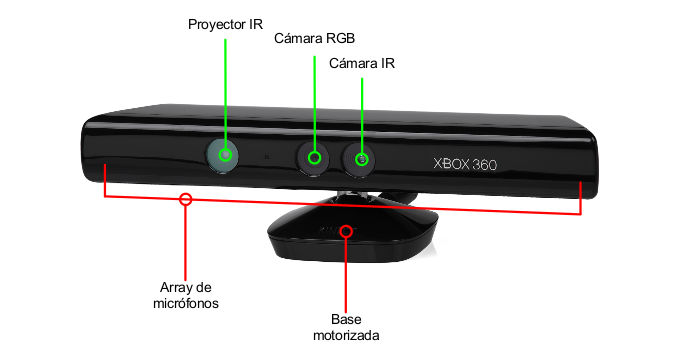
\includegraphics[width=\imsize]
{kinect}
\caption{Microsoft Kinect.}
\label{fig:kinect}
\end{figure}

\section{Descripcion}
\label{sec:descripcion-kinect}
La camara RGB produce un stream de datos de 24 bits por pixel, 8 bits por cada color. Su resolucion estandar es 640x480 pixels con una tasa de muestreo maxima de 30 FPS. \\
El sensor de profundidad esta compuesto por un emisor laser infrarrojo y un sensor CMOS monocromo. Produce un stream de datos de 11 bits. Posee una resolucion estandar de 640x480 pixels a una tasa de muestreo maxima de 30 FPS. \\
El campo de vision es de 57° horizontal y 43° vertical. \\
El resto de los sensores asi como el mecanismo de inclinacion no se exponen este trabajo debido a que no son relevantes para el funcionamiento de la aplicacion.

\section{Funcionamiento interno}
\label{sec:funcionamiento-kinect}

El funcionamiento de la camara Kinect esta basado en tecnologia propiedad de la empresa israeli PrimeSense \cite{primesense}. \\
Para obtener una imagen de profundidad el emisor laser emite un patron de puntos que es capturado por la camara infrarroja (sensor CMOS monocromo). AGREGAR FIGURA. \\
El proceso que se describe en la patente CITAR[PrimeSensePatent] esta formado por las siguientes etapas :
\begin{enumerate}
\item Capturar el patron de puntos para un conjunto de imagenes de referencia a diferentes distancias del plano del sensor.
\item Capturar el patron de puntos sobre una imagen de test de la region de interes.
\item Encontrar la imagen de referencia que mayor similitud tiene con la imagen de test utilizando un metodo de Correlacion Cruzada \cite[wiki:cross-correlation].
\item Estimar el mapa 3D de la escena por medio de un proceso de triangulacion utilizando los desplazamientos entre la imagen de test y la imagen de referencia elegida. 
\end{enumerate}

En el caso del Microsoft Kinect, las imagenes de referencia han sido capturadas contra una superficie plana a distancias predifinidas y estan almacenadas en el dispositivo. El sensor devuelve la imagen de profundidad en forma de valores de disparidad que luego son traducidos a distancias en metros [VER: o milimitros], en un procedimento externo, mediante la conversion : AGREGAR FORMULA.

AGREGAR QUE LA IMAGEN DE PROFUNDIDAD ESTA SINCRONIZADA CON LA IMAGEN DE RGB QUE FUE PROCESADA CON UN FILTRO DE BAYER.


\section{Consideraciones}
\label{sec:consideraciones-kinect}

Su rango util es de 0.4 a 4 metros.
Algunas consideraciones especiales a tener en cuenta. LUZ, SUPERFICIE REFLECTANTES, RELACION DISTANCIA - ERROR.